\documentclass[aspectratio=169, 10pt]{beamer} % 16:9 aspect ratio (modern standard)

% --- PACKAGES ---
\usepackage[utf8]{inputenc}
\usepackage[T1]{fontenc}
\usepackage[ngerman]{babel}
\usepackage{lmodern} % Improved font quality
\usepackage{helvet}  % Helvetica as sans-serif font (looks more modern)
\usepackage{graphicx}
% Search paths for images (cover both in-place and outdir builds)
\graphicspath{{images/}{./images/}{../images/}}
\renewcommand{\familydefault}{\sfdefault} % Set sans-serif as default

\usepackage{booktabs} % Nice table rules
\usepackage{siunitx}  % For units
\usepackage{graphicx}
\usepackage{tikz}     % For drawings and diagrams
\usepackage[most]{tcolorbox}
\usepackage{pgfplots}
\pgfplotsset{compat=1.18}
\usetikzlibrary{shapes, arrows, arrows.meta, positioning, shadows, calc, fit, backgrounds}
\usepackage{fontawesome5} % For modern icons
\usepackage{xcolor}
\usepackage{colortbl} % For colored table cells

% --- THEME & COLORS (MODERN FLAT DESIGN) ---
\usetheme{Madrid} % Madrid is clean, but we customize it heavily
\usecolortheme{default}

% Define custom color palette (DHBW Red or a Tech Blue)
\definecolor{PrimaryColor}{RGB}{44, 62, 80}    % Dark Blue (Midnight Blue)
\definecolor{SecondaryColor}{RGB}{44, 62, 80} % Accent Color
\definecolor{LightGray}{RGB}{236, 240, 241}    % Light Background
\definecolor{TechGreen}{RGB}{39, 174, 96}      % For Success/Progress

% Set Beamer colors
\setbeamercolor{palette primary}{bg=PrimaryColor,fg=white}
\setbeamercolor{palette secondary}{bg=PrimaryColor!80,fg=white}
\setbeamercolor{palette tertiary}{bg=PrimaryColor!90,fg=white}
\setbeamercolor{structure}{fg=PrimaryColor} % Heading color
\setbeamercolor{frametitle}{bg=PrimaryColor,fg=white}
\setbeamercolor{title}{bg=PrimaryColor,fg=white}

% Modernize blocks (Flat, no shadows)
\setbeamertemplate{blocks}[rounded][shadow=false]
\setbeamercolor{block title}{bg=PrimaryColor!15,fg=PrimaryColor}
\setbeamercolor{block body}{bg=PrimaryColor!5,fg=black}
\setbeamercolor{block title alerted}{bg=SecondaryColor!15,fg=SecondaryColor}
\setbeamercolor{block body alerted}{bg=SecondaryColor!5,fg=black}

% Hide navigation symbols (looks cleaner)
\setbeamertemplate{navigation symbols}{}

% Customize itemize bullets
\setbeamertemplate{itemize item}{\color{SecondaryColor}$\blacksquare$}
\setbeamertemplate{itemize subitem}{\color{SecondaryColor}\scriptsize$\blacktriangleright$}

% Minimalist footer
\setbeamertemplate{footline}{
  \leavevmode%
  \hbox{%
  \begin{beamercolorbox}[wd=.333333\paperwidth,ht=2.25ex,dp=1ex,center]{author in head/foot}%
    \usebeamerfont{author in head/foot}\insertshortauthor
  \end{beamercolorbox}%
  \begin{beamercolorbox}[wd=.333333\paperwidth,ht=2.25ex,dp=1ex,center]{title in head/foot}%
    \usebeamerfont{title in head/foot}\insertshorttitle
  \end{beamercolorbox}%
  \begin{beamercolorbox}[wd=.333333\paperwidth,ht=2.25ex,dp=1ex,rightskip=2ex]{date in head/foot}%
    \usebeamerfont{date in head/foot}\insertshortdate{}\hspace*{2em}
    \insertframenumber{} / \inserttotalframenumber
  \end{beamercolorbox}}%
  \vskip0pt%
}

% --- CUSTOM COMMANDS ---
% Command for visual progress bars in tables
\newcommand{\progressbar}[1]{%
    \begin{tikzpicture}
        \fill[LightGray] (0,0) rectangle (1.5,0.25);
        \fill[TechGreen] (0,0) rectangle (#1*0.015,0.25);
    \end{tikzpicture}%
}

% --- METADATA ---
\title[6-Achs-Slicer]{Prototypische Entwicklung eines 6-Achs-Slicers}
\subtitle{für nichtplanare, robotergestützte additive Fertigung}
\author[Axtmann, Wachsmann, Stahl]{Adrian Axtmann \and Nik Wachsmann \and Ben Stahl}
\institute[DHBW]{Studiengang Informatik \ DHBW Karlsruhe}
\date{\today}
% DHBW Logo
\titlegraphic{
\includegraphics[height=1.2cm]{dhbw_Logo.png}}

\begin{document}

% --- TITLE PAGE ---
{
\setbeamertemplate{footline}{} % No footer on title page
\begin{frame}
    \titlepage
\end{frame}
}

% --- AGENDA ---
\begin{frame}{Agenda}
    \tableofcontents[hideallsubsections]
\end{frame}

% --- CONTENT (one file per section) ---
% \begin{frame}{Unser Team}
    \begin{columns}[T,onlytextwidth]
        \column{0.33\textwidth}
            \centering
            \begin{tikzpicture}
                \node[circle, draw=PrimaryColor!45, fill=LightGray, minimum size=2.3cm, line width=1pt] (p1) {\Huge \faUser};
                \node[below=0.2cm of p1, align=center] {\textbf{Adrian Axtmann}};
            \end{tikzpicture}
        \column{0.33\textwidth}
            \centering
            \begin{tikzpicture}
                \node[circle, draw=PrimaryColor!45, fill=LightGray, minimum size=2.3cm, line width=1pt] (p2) {\Huge \faUser};
                \node[below=0.2cm of p2, align=center] {\textbf{Nik Wachsmann}};
            \end{tikzpicture}
        \column{0.33\textwidth}
            \centering
            \begin{tikzpicture}
                \node[circle, draw=PrimaryColor!45, fill=LightGray, minimum size=2.3cm, line width=1pt] (p3) {\Huge \faUser};
                \node[below=0.2cm of p3, align=center] {\textbf{Ben Stahl}};
            \end{tikzpicture}
    \end{columns}
\end{frame}
\section{Motivation}

\begin{frame}{Warum 6-Achs-Druck?}
    \begin{columns}[T]
        \column{0.6\textwidth}
            \textbf{Limitierungen klassischer 3-Achs-Verfahren:}
            \begin{itemize}
                \item Schichten müssen parallel zur Bauplattform sein.
                \item Treppenstufeneffekte auf gekrümmten Oberflächen.
                \item Hoher Bedarf an Stützstrukturen bei Überhängen.
                \item Mechanische Schwäche entlang der Schichtgrenzen.
            \end{itemize}
            
            \vspace{0.25cm}
            \textbf{Potential von 6 Achsen:}
            \begin{itemize}
                \item \textcolor{SecondaryColor}{\textbf{Nichtplanares Slicen:}} 
                    Erhöhte Stabilität durch nicht-parallele und nicht-planare Schichten.
                \item \textcolor{SecondaryColor}{\textbf{Support-Reduktion:}} 
                    Überhänge ohne Stütze durch Änderung der Druckrichtung.
                \item \textcolor{SecondaryColor}{\textbf{Oberflächenqualität:}}
                    Glattere Oberflächen durch Anpassung der Schichtgeometrie an die Modellkonturen.
            \end{itemize}

        \column{0.4\textwidth}
            % Vergleichsgrafik: Treppe vs Smooth
            \centering
            \begin{tcolorbox}[
                enhanced, colback=white, colframe=PrimaryColor!30, arc=2mm, boxrule=0.5pt,
                title={Planar (3-Achs)}, fonttitle=\bfseries\tiny, coltitle=PrimaryColor, colbacktitle=PrimaryColor!10
            ]
                \centering
                \begin{tikzpicture}[scale=0.5]
                    \draw[gray!50] (0,0) -- (3,1.5); % Slope
                    \foreach \x in {0,0.5,...,2.5} {
                        \draw[fill=PrimaryColor!40] (\x, {0.5*\x}) rectangle (\x+0.6, {0.5*\x+0.25});
                    }
                \end{tikzpicture}
            \end{tcolorbox}
            
            \vspace{0.2cm}

            \begin{tcolorbox}[
                enhanced, colback=white, colframe=SecondaryColor!30, arc=2mm, boxrule=0.5pt,
                title={Nichtplanar (6-Achs)}, fonttitle=\bfseries\tiny, coltitle=SecondaryColor, colbacktitle=SecondaryColor!10
            ]
                \centering
                \begin{tikzpicture}[scale=0.5]
                    \draw[fill=SecondaryColor!40, draw=SecondaryColor] (0,0) -- (3,1.5) -- (3,2.0) -- (0,0.5) -- cycle;
                \end{tikzpicture}
            \end{tcolorbox}
    \end{columns}
\end{frame}

\section{Übersicht über das Projekt}

\begin{frame}{Übersicht}

    \begin{alertblock}{Vision}
        Entwickling eines neuartigen, 6-Achs-Druckverfahrens, das mithilfe eines Roboterarms 
        komplexe Geometrien mit verbesserter Stabilität und reduzierten Stützstrukturen ermöglicht.
    \end{alertblock}


    \vspace{0.5cm}
    
    \begin{columns}[T]
        \column{0.25\textwidth}
            \centering
            \textbf{Input}\\
            \vspace{0.2cm}
            \faFileCode[regular] \ STL / OBJ\\
            (CAD Modell)
            
        \column{0.25\textwidth}
            \centering
            \textbf{Slice-Logic}\\
            \vspace{0.2cm}
            \faCogs \ Slicing\\
            (Medusa)
        
        \column{0.25\textwidth}
            \centering
            \textbf{Kinematik}\\
            \vspace{0.2cm}
            \faCogs \ Toolpath \\
            (Kronos)

        \column{0.25\textwidth}
            \centering
            \textbf{Output}\\
            \vspace{0.2cm}
            \faRobot \ Print Part \\
            (Robotersteuerung)
    \end{columns}
\end{frame}


\section{Vorstellung Medusa}

\begin{frame}{Medusa}
    \centering
    \textit{Multi‑dimensional Extrusion \& Dimensional Unified Slicing Algorithm}
    \vspace{0.4cm}

    \begin{columns}[T]
        \column{0.33\textwidth}
            \centering
            \faFileCode\\
            \textbf{Modell‑Darstellung}\\
            \small Import \& Visualisierung (STL/OBJ)
        \column{0.33\textwidth}
            \centering
            \faCogs\\
            \textbf{Slicing}\\
            \small Nichtplanare, parametrische Schichten
        \column{0.33\textwidth}
            \centering
            \faRobot\\
            \textbf{Pfad‑Generierung}\\
            \small 6‑Achs Toolpaths \& Ausgabeformate
    \end{columns}

    \vspace{0.35cm}
    \begin{block}{Kernaufgaben}
        \small
        \begin{itemize}
            \item Robustes Mesh‑Handling und Visual Debugging
            \item Modulare Slicing‑Pipeline (austauschbar)
            \item Integration mit KRONOS für Kinematik und Collision‑Checks
        \end{itemize}
    \end{block}
\end{frame}

    \begin{frame}{Medusa: Architektur \& Modulaufbau}
        \textbf{Layered Architektur:}
        \begin{itemize}
            \item \textbf{App}: Einstiegspunkt, Window/Main-Loop, Orchestrierung
            \item \textbf{UI (ImGui)}: Panels, File-Browser, Parameter/Settings
            \item \textbf{Graphics (OpenGL)}: Mesh, Shader, Renderer, Scene
            \item \textbf{Controls}: Input-Handling (Kamera/Model-Controller)
            \item \textbf{Slicing (geplant)}: Slicing-Pipeline \& 6-Achs Toolpaths
            \item \textbf{Core}: Logger, Camera, Math/Utilities (wiederverwendbar)
        \end{itemize}

        \vspace{0.35cm}
        \textbf{Kopplung/Prinzipien:}
        \begin{itemize}
            \item klare Modulgrenzen, erweiterbare Pipeline (Slicing austauschbar)
            \item Dependencies via CMake FetchContent (kein manuelles Setup)
        \end{itemize}
    \end{frame}

    \begin{frame}{Medusa: Architektur (Diagramm)}
        \centering
        \begin{tikzpicture}[
            font=\scriptsize,
            box/.style={draw=SecondaryColor, thick, rounded corners, align=center, minimum width=3.6cm},
            layer/.style={box, fill=SecondaryColor!8, minimum height=0.75cm},
            core/.style={box, fill=SecondaryColor!14, minimum height=0.75cm},
            ext/.style={box, fill=SecondaryColor!5, minimum height=0.75cm},
            mod/.style={box, fill=SecondaryColor!10, minimum height=0.6cm, minimum width=1.65cm},
            arrow/.style={->, thick, SecondaryColor!70}
        ]
            \node[layer] (app) {Application\\\texttt{src/app}};
            \node[mod, below left=0.6cm and 1.5cm of app.south] (controls) {Controls\\\texttt{src/controls}};
            \node[mod, below=0.6cm of app.south] (graphics) {Graphics\\\texttt{src/graphics}};
            \node[mod, below right=0.6cm and 1.5cm of app.south] (ui) {UI\\\texttt{src/ui}};

            \node[mod, below=0.25cm of graphics.south] (slicing) {Slicing (planned)\\\texttt{src/slicing}};
            \node[core, below=0.6cm of slicing.south, minimum width=6.8cm] (core) {Core\\Logger \textbar\ Camera \textbar\ Math\\\texttt{src/core}};
            \node[ext, below=0.6cm of core.south, minimum width=8.5cm] (ext) {External Libraries\\GLFW \textbar\ GLAD \textbar\ GLM \textbar\ ImGui \textbar\ Assimp \textbar\ spdlog};

            \draw[arrow] (app) -- (controls);
            \draw[arrow] (app) -- (graphics);
            \draw[arrow] (app) -- (ui);
            \draw[arrow] (graphics) -- (slicing);
            \draw[arrow] (controls) -- (core);
            \draw[arrow] (ui) -- (core);
            \draw[arrow] (slicing) -- (core);
            \draw[arrow] (core) -- (ext);
        \end{tikzpicture}
    \end{frame}
    
    \begin{frame}{Code Overview}
        \small
        \begin{columns}
            \column{0.55\textwidth}
                \begin{itemize}
                    \item \textbf{Total files:} 67
                    \item \textbf{Total lines of code:} 4\,286
                \end{itemize}

            \column{0.45\textwidth}
                \begin{tabular}{@{}l r@{}}
                \textbf{Language} & \textbf{LOC} \\\hline
                C++ & 2\,492 \\
                CMake & 786 \\
                C/C++ Header & 411 \\
                Markdown & 286 \\
                YAML & 257 \\
                Dockerfile & 54 \\\hline
                \textbf{SUM} & \textbf{4\,286}
                \end{tabular}
        \end{columns}
    \end{frame}

\section{Vorstellung Kronos}

\begin{frame}{Kronos: Kinematic Robotic Operations \& Navigation Orchestration System}
    \begin{alertblock}{Überblick}
        Kronos ist die Kinematik- und Pfadplanungs-Engine unseres 6-Achs-Slicers. 
        Es übersetzt die Druckpfade von Medusa in präzise Bewegungsbefehle für den Roboterarm, 
        um eine genaue und effiziente Fertigung zu gewährleisten.
    \end{alertblock}

    \vspace{0.25cm}
    \textbf{Funktionsweise von Kronos:}
    \begin{itemize}
        \item \textbf{Inverse Kinematik (IK):} Berechnet die 6 Gelenkwinkel $(J1...J6)$ für eine gegebene TCP-Position und Orientierung.
        \item \textbf{Pfad-Interpolation:} Stellt sicher, dass Bewegungen zwischen zwei Punkten linear im kartesischen Raum sind.
        \item \textbf{Singularitäts-Schutz:} Vermeidet Konfigurationen, bei denen der Roboter unendliche Geschwindigkeiten benötigen würde.
        \item \textbf{Dynamische Anpassung:} Passt die Druckparameter in Echtzeit an, um Materialfluss und Druckqualität zu optimieren.
    \end{itemize}
\end{frame}

\begin{frame}{Kronos Entwicklungsumgebung} % Docker-Container mit ROS, MoveIt, Gazebo
    \begin{alertblock}{Entwicklungsumgebung}
        Kronos wird in einem Docker-Container entwickelt, der ROS (Robot Operating System), MoveIt und Gazebo enthält. 
        Diese Tools ermöglichen die Simulation und Steuerung von Roboterarmen, die Entwicklung von Pfadplanungsalgorithmen und die Integration von Sensoren für die Echtzeit-Überwachung.
    \end{alertblock}

    \vspace{0.5cm}
    \textbf{Vorteile der Docker-basierten Entwicklung:}
    \begin{itemize}
        \item Konsistente Entwicklungsumgebung über verschiedene Systeme hinweg.
        \item Einfache Verwaltung von Abhängigkeiten und Bibliotheken.
        \item Möglichkeit zur schnellen Iteration und Fehlerbehebung durch isolierte Container.
    \end{itemize}
\end{frame}

\section{Slicing-Algorithmen}

\begin{frame}{Slicing-Algorithmen}
    \begin{description}
        \item[Sphären-Algorithmus] 
        Sphärenförmige Ausbreitung ausgehend von einem Startpunkt.
        \vspace{0.5cm}
        \item[Base-Algorithmus] 
        Planares Slicing entlang einer sich ändernden Normalen.
        \vspace{0.5cm}
        \item[Kristall-Algorithmus] 
        Kombination aus Sphären- und Base-Algorithmus.
    \end{description}
\end{frame}

\begin{frame}{Sphären-Algorithmus}
    \begin{columns}[T]
        % Linke Spalte für den Text
        \begin{column}{0.6\textwidth}
            \begin{itemize}
                \item Ausbreitung in Sphären um einen Startpunkt.
                \vspace{0.5cm}
                \item Wahl eines neuen Startpunkts anhand der Druckernormalen.
            \end{itemize}
        \end{column}

        % Rechte Spalte für das Bild
        \begin{column}{0.4\textwidth}
            \centering
            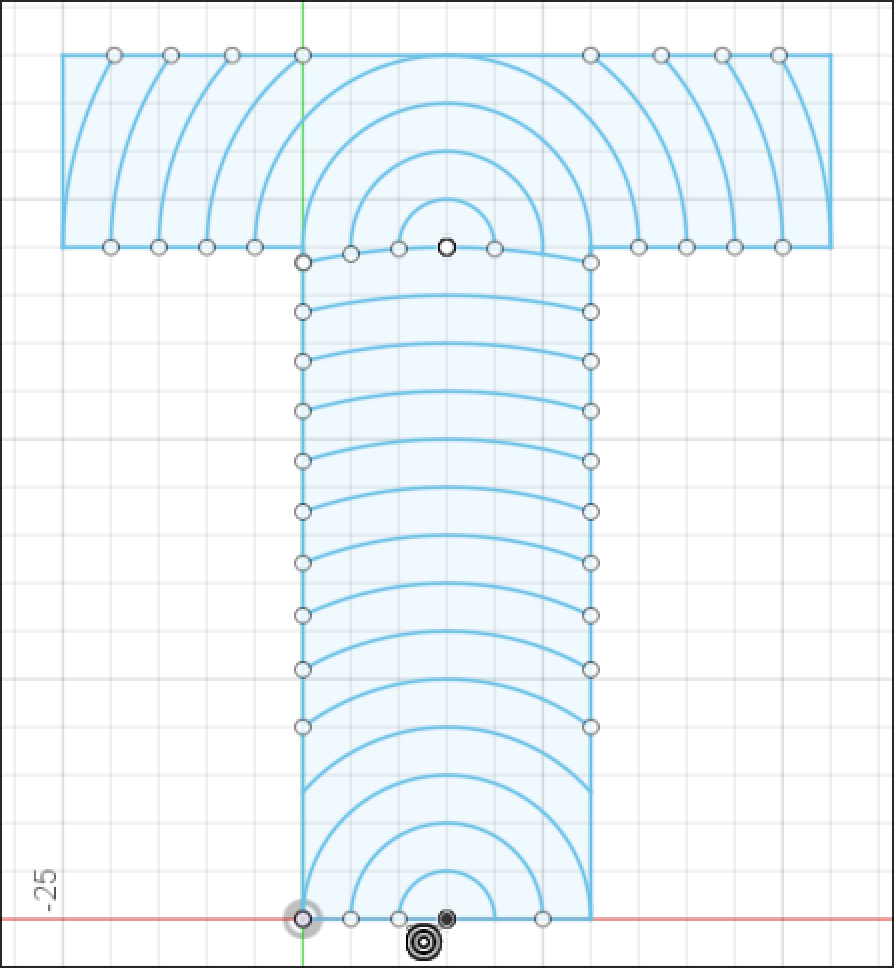
\includegraphics[width=\textwidth]{images/sphere.png}
        \end{column}
    \end{columns}
\end{frame}

\begin{frame}{Base-Algorithmus}
    \begin{columns}[T]
        % Linke Spalte für den Text
        \begin{column}{0.6\textwidth}
            \begin{itemize}
                \item Wahl einer Startnormalen.
                \vspace{0.5cm}
                \item Planares Slicing entlang der Normalen.
                \vspace{0.5cm}
                \item Wahl einer neuen Normalen bei einem Überhang.
            \end{itemize}
        \end{column}

        % Rechte Spalte für das Bild
        \begin{column}{0.4\textwidth}
            \centering
            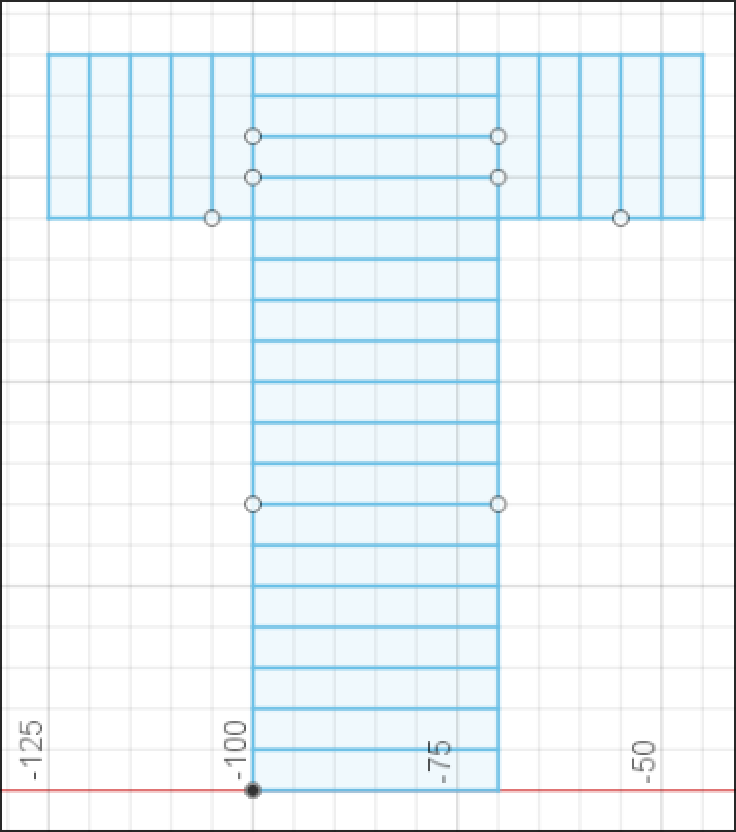
\includegraphics[width=\textwidth]{images/base.png}
        \end{column}
    \end{columns}
\end{frame}

\begin{frame}{Kristall-Algorithmus}
    \begin{columns}[T]
        % Linke Spalte für den Text
        \begin{column}{0.6\textwidth}
            \begin{itemize}
                \item Kombination aus Sphären- und Base-Algorithmus.
                \vspace{0.5cm}
                \item Wahl einer Startnormalen und planares Slicing entlang der Normalen.
                \vspace{0.5cm}
                \item Frühzeitige Erkennung eines Überhanges.
                \vspace{0.5cm}
                \item Langsames Aufbauen einer Sphäre.
            \end{itemize}
        \end{column}

        % Rechte Spalte für das Bild
        \begin{column}{0.4\textwidth}
            \centering
            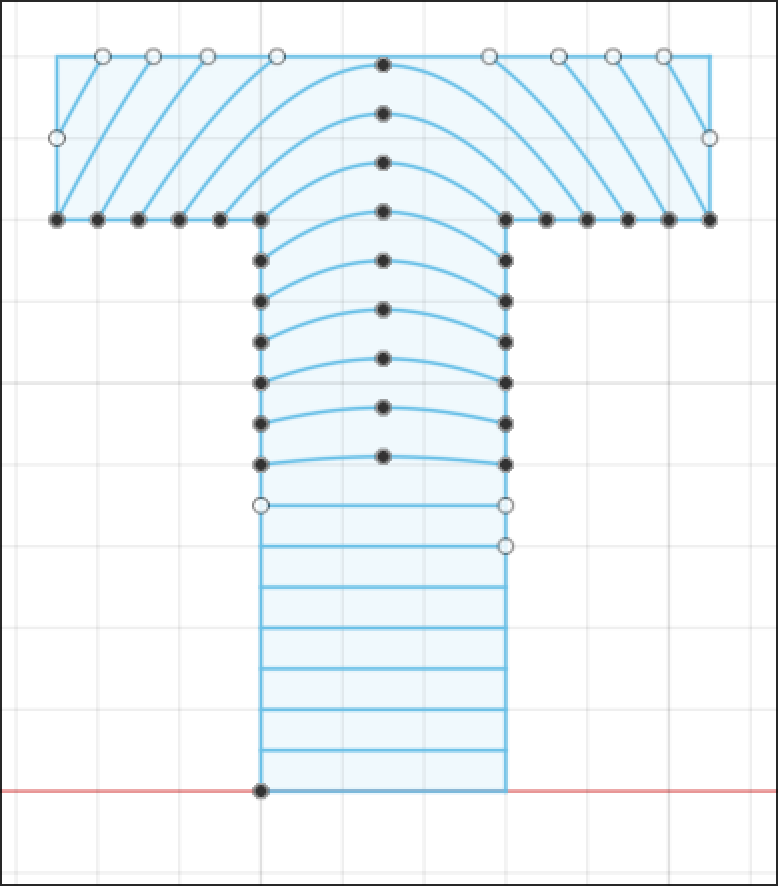
\includegraphics[width=\textwidth]{images/kristall.png}
        \end{column}
    \end{columns}
\end{frame}

\begin{frame}{Testmodelle}
    \centering
    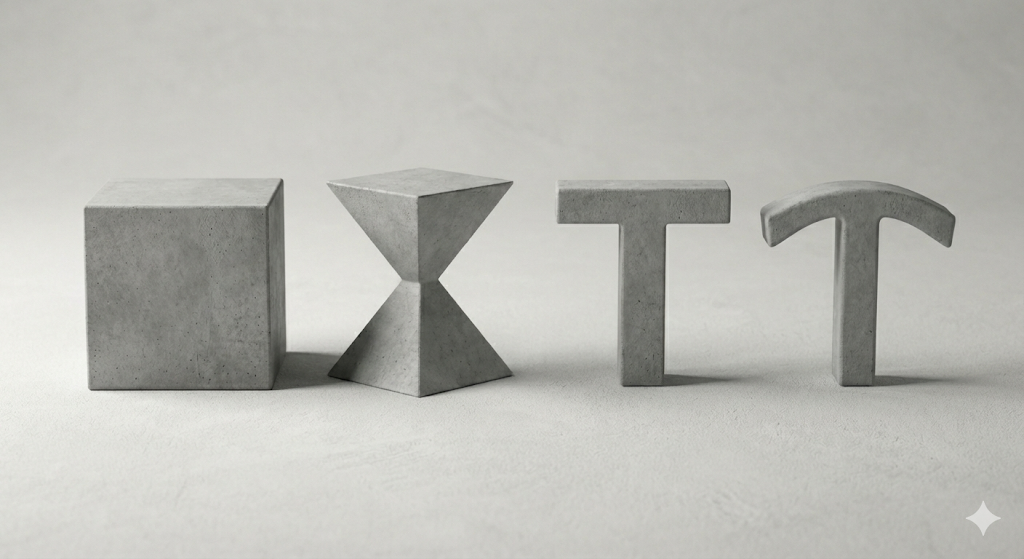
\includegraphics[width=0.75\textwidth]{images/models.png}
\end{frame}
\section{Nächste Schritte und Ziel}

\begin{frame}{Nächste Schritte}
    \begin{itemize}
        \item Finalisierung der Schnittstelle Medusa $\leftrightarrow$ Kronos.
        \vspace{0.2cm}
        \item Implementierung eines testweisen Slicing-Algorithmus in Medusa.
        \vspace{0.2cm}
        \item Steuerung des UR-3e über Kronos.
    \end{itemize}
\end{frame}

\begin{frame}{Projektziel}
    \begin{itemize}
        \item Slicing eines 3D-Modells in nichtplanare Schichten.
        \vspace{0.2cm}
        \item Generierung von Robotertrajektorien für die additive Fertigung.
        \vspace{0.2cm}
        \item Simulation und Steuerung eines UR-3e Roboters für den Druckprozess.
        \vspace{0.2cm}
        \item Durchführung von Drucktests an einem realen Roboter.
    \end{itemize}
\end{frame}
\begin{frame}{Fragen}
    \centering
    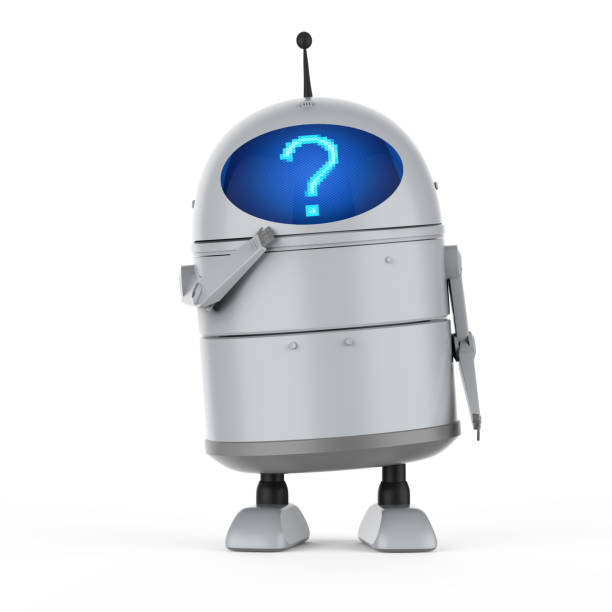
\includegraphics[width=0.4\textwidth]{images/questionmark.jpg}
\end{frame}

\end{document}
